\section{Deskriptive Statistik}

\subsection{Begriffe}

\begin{concept}{Grundlegende Begriffe}

\begin{minipage}{0.4\linewidth}
\begin{itemize}
    \item $\Omega =$ Grundgesamtheit
    \item $n =$ Anzahl Objekte
    \item $X =$ Stichprobenwerte
    \item $a =$ Ausprägungen
    \item $h =$ Absolute Häufigkeit
    \item $f =$ Relative Häufigkeit
\end{itemize}
\end{minipage}
\begin{minipage}{0.6\linewidth}
    \vspace{-6mm}
    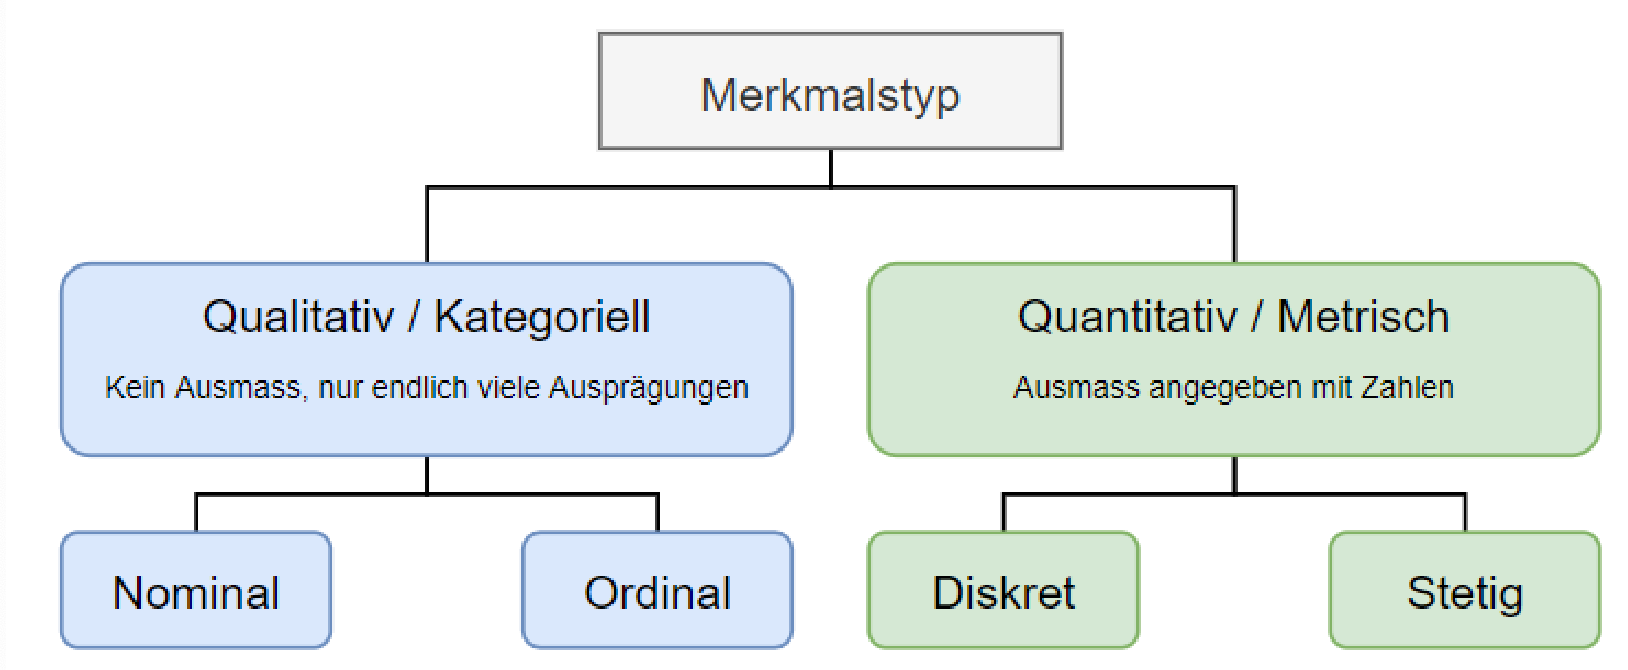
\includegraphics[width=\linewidth]{images/merkmalstypen.png}
\end{minipage}

\begin{itemize}
    \item $H =$ Kumulative Absolute Häufigkeit
    \item $F =$ Kumulative Relative Häufigkeit
\end{itemize}
\end{concept}

\begin{definition}{Statistische Grundbegriffe}
\begin{itemize}
    \item \textbf{Merkmalsträger/Statistische Einheiten}: Objekte, an denen interessierende Grössen beobachtet werden
    \item \textbf{Grundgesamtheit}: Alle statistischen Einheiten, über die Aussagen gewonnen werden sollen
    \item \textbf{Vollerhebung}: Eigenschaften werden bei jedem Individuum in der Grundgesamtheit erhoben
    \item \textbf{Stichprobe}: Untersuchte Teilmenge der Grundgesamtheit (repräsentativ)
    \item \textbf{Merkmal}: Interessierende Grösse, die an den Einheiten beobachtet wird
\end{itemize}
\end{definition}

\begin{concept}{Merkmalstypen}
\begin{itemize}
    \item \textbf{Qualitativ/Kategoriell}: Ausprägung und kein Ausmass (endlich viele Ausprägungen)
    \begin{itemize}
        \item \textbf{Nominal}: Reine Kategorisierung (z.B. Parteien bei Wahlen)
        \item \textbf{Ordinal}: Ordnung vorhanden (z.B. Schulnoten)
    \end{itemize}
    \item \textbf{Quantitativ/Metrisch}: Ausmass wird mit Zahlen angegeben
    \begin{itemize}
        \item \textbf{Diskret}: Abzählbar viele Ausprägungen (z.B. Würfelwurf)
        \item \textbf{Stetig}: Alle Ausprägungen in einem reellen Intervall (z.B. Länge)
    \end{itemize}
\end{itemize}
\end{concept}




\subsection{Häufigkeiten und Verteilungsfunktionen (PMF, CDF)}

\subsubsection{Absolute und relative Häufigkeiten}

\begin{minipage}{0.5\columnwidth}
\begin{formula}{Absolute Häufigkeit H}
\vspace{-2mm}\\
    %TODO: H(X) ??
$$
H=\sum_{i=1}^{n} h_{i}
$$
\\
\small{
$h_{i}$: Einzelhäufigkeit der\\ $i$-ten Beobachtung \\
$n$: Anzahl der Beobachtungen.}
\end{formula}
\end{minipage}
\begin{minipage}{0.5\columnwidth}
\begin{formula}{Relative Häufigkeit F}
    \vspace{-2mm}\\
$$
F=\sum_{i=1}^{n} f_{i}, \quad F(x)=\frac{H(x)}{n}
$$
\small{
$f_{i}$: Einzelrelative Häufigkeit der\\ $i$-ten Beobachtung \\
$H(x)$: Absolute Häufigkeit eines\\ Wertes $x$}
\end{formula}
\end{minipage}

\raggedcolumns

\subsubsection{Kumulative Verteilungsfunktion (CDF)}
%TODO: complete with info from script and correctly structure

\begin{definition}{Nicht klassierte Daten (PMF und CDF)}\\
Die absolute Häufigkeit kann als Funktion $h: \mathbb{R} \rightarrow \mathbb{R}$ bezeichnet werden.
$$
h_{i}
$$
\\
$h_{i}$: Absolute Häufigkeit der $i$-ten Beobachtung.
\\
\\
Die relative Häufigkeit kann als Funktion $f: \mathbb{R} \rightarrow \mathbb{R}$ bezeichnet werden.
$$
f_{i}=\frac{h_{i}}{n}
$$
\\
$f_{i}$: Relative Häufigkeit der $i$-ten Beobachtung, \\
$h_{i}$: Absolute Häufigkeit der $i$-ten Beobachtung, \\
$n$: Anzahl der Beobachtungen.
\end{definition}

\begin{KR}{Erstellen einer Häufigkeitsverteilung}
\begin{enumerate}
    \item Sammle alle verschiedenen Werte
    \item Zähle absolute Häufigkeiten:
        \begin{itemize}
            \item Wie oft kommt jeder Wert vor?
        \end{itemize}
    \item Berechne relative Häufigkeiten:
        \begin{itemize}
            \item Teile jede absolute Häufigkeit durch $n$
        \end{itemize}
    \item Berechne kumulative Häufigkeiten:
        \begin{itemize}
            \item Absolute: Summiere $h_i$ von links nach rechts
            \item Relative: Summiere $f_i$ von links nach rechts
        \end{itemize}
\end{enumerate}
\end{KR}

\subsection{Verteilungsfunktionen für diskrete und stetige Daten}

\begin{concept}{Unterschied zwischen PMF und PDF}
\begin{itemize}
    \item \textbf{PMF (Probability Mass Function)}:
        \begin{itemize}
            \item Für diskrete Daten
            \item Wahrscheinlichkeit für exakte Werte
            \item Summe aller Wahrscheinlichkeiten = 1
        \end{itemize}
    \item \textbf{PDF (Probability Density Function)}:
        \begin{itemize}
            \item Für stetige Daten
            \item Fläche unter Kurve gibt Wahrscheinlichkeit
            \item Integral über gesamten Bereich = 1
        \end{itemize}
\end{itemize}
\end{concept}

\begin{definition}{Diskrete Verteilungsfunktionen}\\
Die absolute Häufigkeit kann als Funktion $h: \mathbb{R} \rightarrow \mathbb{R}$ bezeichnet werden:
$$h_i$$

Die relative Häufigkeit kann als Funktion $f: \mathbb{R} \rightarrow \mathbb{R}$ bezeichnet werden:
$$f_i = \frac{h_i}{n}$$
\end{definition}

\begin{example2}{Diskrete Häufigkeitsverteilung}\\
\renewcommand{\arraystretch}{2}%
\begin{center}
\begin{tabular}{|c|c|c|c|c|c|}
\hline
$a_i$ & 397 & 398 & 399 & 400 & Total \\
\hline
$h_i$ & 1 & 3 & 7 & 5 & 16 \\
\hline
$f_i$ & $\frac{1}{16}$ & $\frac{3}{16}$ & $\frac{7}{16}$ & $\frac{5}{16}$ & 1 \\
\hline
$H_i$ & 1 & 4 & 11 & 16 & \\
\hline
$F_i$ & $\frac{1}{16}$ & $\frac{4}{16}$ & $\frac{11}{16}$ & $\frac{16}{16}$ & \\
\hline
\end{tabular}
\end{center}
\end{example2}

\subsection{Klassierte Stichproben}


\begin{definition}{Häufigkeiten bei nicht-klassierten Daten}
\begin{itemize}
    \item \textbf{Absolute Häufigkeit} $h_i$: Anzahl Vorkommen des Wertes $a_i$
    \item \textbf{Relative Häufigkeit} $f_i$: $f_i = \frac{h_i}{n}$
    \item \textbf{Kumulative absolute Häufigkeit} $H_i$: $H_i = \sum_{j=1}^i h_j$
    \item \textbf{Kumulative relative Häufigkeit} $F_i$: $F_i = \sum_{j=1}^i f_j = \frac{H_i}{n}$
\end{itemize}
\end{definition}

\begin{definition}{Häufigkeiten bei klassierten Daten}
Bei grossen Stichproben metrisch stetiger Merkmale werden die Werte in Klassen eingeteilt:
\begin{itemize}
    \item Klassen sind aneinandergrenzende Intervalle
    \item Obere Intervallgrenzen gehören zum nächsten Intervall
    \item Relative Häufigkeit einer Klasse = Anzahl Werte in Klasse / Stichprobengrösse
    \item Relative Häufigkeitsdichte = Relative Häufigkeit / Klassenbreite
\end{itemize}
\end{definition}

\begin{KR}{Klasseneinteilung}
\textbf{Faustregeln:}
\begin{itemize}
    \item Klassen sollten gleich breit gewählt werden
    \item Anzahl Klassen zwischen 5 und 20
    \item Anzahl Klassen sollte $\sqrt{n}$ nicht überschreiten
    \item Klassenbreite = $\frac{\text{Max - Min}}{\text{Anzahl Klassen}}$
\end{itemize}
\end{KR}

\begin{example2}{Häufigkeitsverteilung}
Noten einer Klasse: 3.5, 4.0, 4.0, 4.5, 4.5, 4.5, 5.0, 5.0, 5.5, 6.0
\begin{itemize}
    \item $n = 10$ (Stichprobengrösse)
    \item Absolute Häufigkeiten: $h_{3.5}=1$, $h_{4.0}=2$, $h_{4.5}=3$, $h_{5.0}=2$, $h_{5.5}=1$, $h_{6.0}=1$
    \item Relative Häufigkeiten: $f_{3.5}=0.1$, $f_{4.0}=0.2$, $f_{4.5}=0.3$, $f_{5.0}=0.2$, $f_{5.5}=0.1$, $f_{6.0}=0.1$
    \item Kumulative absolute Häufigkeiten: $H_{3.5}=1$, $H_{4.0}=3$, $H_{4.5}=6$, $H_{5.0}=8$, $H_{5.5}=9$, $H_{6.0}=10$
\end{itemize}
\end{example2}

\begin{KR}{Klassenbildung für stetige Daten}
\begin{enumerate}
    \item Bestimme Spannweite (Max - Min)
    \item Wähle Anzahl Klassen $k$:
        \begin{itemize}
            \item $5 \leq k \leq 20$
            \item $k \leq \sqrt{n}$
        \end{itemize}
    \item Berechne Klassenbreite:
        \begin{itemize}
            \item $d = \frac{\text{Spannweite}}{k}$
            \item Runde auf praktische Zahl
        \end{itemize}
    \item Bestimme Klassengrenzen:
        \begin{itemize}
            \item Start bei Min oder praktischem Wert darunter
            \item Ende bei Max oder praktischem Wert darüber
        \end{itemize}
    \item Zähle Häufigkeiten in jeder Klasse
\end{enumerate}
\end{KR}

\begin{concept}{Klassenbildung (Faustregeln)}\\
\begin{itemize}
  \item Die Klassen sollten gleich breit gewählt werden
  \item Die Anzahl der Klassen sollte zwischen 5 und 20 liegen, jedoch $\sqrt{n}$ nicht überschreiben
  \item Klassengrenzen sollten 'runde' Zahlen sein
  \item Werte auf Klassengrenzen kommen in die obere Klasse
\end{itemize}
\end{concept}

\begin{definition}{Stetige Verteilungsfunktionen}\\
Die absolute Häufigkeitsdichtefunktion erhält man, indem der Wert der absoluten Häufigkeit $h_i$ durch die Klassenbreite (Säulenbreite) $d_i$ geteilt wird:
$$h(x) = \frac{h_i}{d_i}$$

Die relative Häufigkeitsdichtefunktion (PDF) $f: \mathbb{R} \rightarrow [0,1]$ erhält man aus der absoluten Häufigkeitsdichtefunktion, indem man den Wert durch die Stichprobengrösse $n$ teilt:
$$\text{PDF} = f(x) = \frac{h(x)}{n}$$
\end{definition}

\begin{example2}{Stetige Häufigkeitsverteilung}
\renewcommand{\arraystretch}{2}%
%TODO make fit
\begin{center}
\begin{tabular}{|c|c|c|c|c|c|}
\hline
Klassen & [100,200) & [200,500) & [500,800) & [800,1000) & Total \\
\hline
$h_i$ & 35 & 182 & 317 & 84 & 618 \\
\hline
$f_i$ & $\frac{35}{618}$ & $\frac{182}{618}$ & $\frac{317}{618}$ & $\frac{84}{618}$ & Area = 1 \\
\hline
$d_i$ & 100 & 300 & 300 & 200 & \\
\hline
$h(x)$ & $\frac{35}{100}$ & $\frac{182}{300}$ & $\frac{317}{300}$ & $\frac{84}{200}$ & \\
\hline
$f(x)$ & $\frac{35}{100 \cdot 618}$ & $\frac{182}{300 \cdot 618}$ & $\frac{317}{300 \cdot 618}$ & $\frac{84}{200 \cdot 618}$ & \\
\hline
\end{tabular}
\end{center}
\end{example2}





\subsection{Kenngrössen}

\subsubsection{Quantile}

\begin{minipage}{0.5\columnwidth}
\begin{definition}{Quantil}
$$
i=\lceil n \cdot q\rceil, \quad Q=x_{i}=x_{\lceil n \cdot q\rceil}
$$
$i$: Position des Quantils, \\
$n$: Anzahl der Beobachtungen, \\
$q$: Quantilswert (z. B. 0.25 für das erste Quartil), \\
$x_{i}$: Beobachtung an Position $i$.
\end{definition}
\end{minipage}
\begin{minipage}{0.5\columnwidth}
\begin{definition}{Interquartilsabstand}
$$
I Q R=Q_{3}-Q_{1}
$$
$IQR$: Interquartilsabstand, \\
$Q_{3}$: Oberes Quartil (75. Perzentil), \\
$Q_{1}$: Unteres Quartil (25. Perzentil).
\end{definition}
\end{minipage}

\begin{KR}{Berechnung von Lagekennwerten}
\begin{enumerate}
    \item Sortiere die Daten aufsteigend
    \item Berechne den Mittelwert:
        \begin{itemize}
            \item Summe aller Werte / Anzahl Werte
        \end{itemize}
    \item Bestimme den Median:
        \begin{itemize}
            \item Bei ungerader Anzahl: mittlerer Wert
            \item Bei gerader Anzahl: Mittelwert der beiden mittleren Werte
        \end{itemize}
    \item Finde den Modus (häufigster Wert)
    \item Berechne die Quartile:
        \begin{itemize}
            \item Q1: 25\%-Quantil
            \item Q2: Median (50\%-Quantil)
            \item Q3: 75\%-Quantil
        \end{itemize}
\end{enumerate}
\end{KR}

\begin{example2}{Berechnung von Quantilen}
Gegeben sei die Datenreihe: 2, 4, 4, 5, 7, 8, 9, 10\\
$n = 8$ Beobachtungen

\textbf{Berechnung Q1 (25\%-Quantil):}
\begin{itemize}
    \item $i = \lceil 8 \cdot 0.25 \rceil = \lceil 2 \rceil = 2$
    \item Q1 = $x_2 = 4$
\end{itemize}

\textbf{Berechnung Q2 (Median):}
\begin{itemize}
    \item $n$ gerade $\rightarrow$ Mittelwert von Position 4 und 5
    \item Q2 = $(5 + 7)/2 = 6$
\end{itemize}

\textbf{Berechnung Q3 (75\%-Quantil):}
\begin{itemize}
    \item $i = \lceil 8 \cdot 0.75 \rceil = \lceil 6 \rceil = 6$
    \item Q3 = $x_6 = 8$
\end{itemize}

\textbf{Interquartilsabstand:}
\begin{itemize}
    \item IQR = Q3 - Q1 = 8 - 4 = 4
\end{itemize}
\end{example2}

\subsubsection{Boxplot}

\begin{definition}{Boxplot}
\vspace{-1mm}\\
\begin{minipage}{0.62\columnwidth}
\begin{itemize}
  \setlength{\itemsep}{1pt}
  \item $\textcolor[HTML]{A70000}{Q_{1}},\textcolor[HTML]{005700}{ Q_{2}=x_{\text {med }}},\textcolor[HTML]{A70000}{ Q_{3}}$ (Quartile)
  \item $I Q R=Q_{3}-Q_{1}$ (Interquartilsabstand)
  \item Untere Antenne $\textcolor[HTML]{0707FF}{x_{u}}:\\ u=\min \left[Q_{1}-1.5 \cdot I Q R, Q_{1}\right]$
  \item Obere Antenne $\textcolor[HTML]{0707FF}{x_{0}}:\\ \quad o=\max \left[Q_{3}+1.5 \cdot I Q R, Q_{3}\right]$
  \item Ausreisser: $\quad x_{i}<\textcolor[HTML]{0707FF}{x_{u}} \vee x_{i}>\textcolor[HTML]{0707FF}{x_{0}}$
\end{itemize}
\end{minipage}
\begin{minipage}{0.35\columnwidth}
  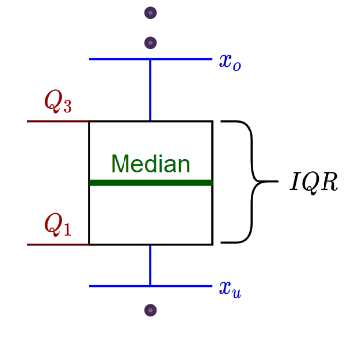
\includegraphics[width=\textwidth]{images/boxplot.png}
\end{minipage}
\end{definition}

\begin{KR}{Erstellen eines Boxplots}
\begin{enumerate}
    \item Berechne die Quartile $Q_1$, $Q_2$ (Median) und $Q_3$
    \item Bestimme den Interquartilsabstand IQR = $Q_3 - Q_1$
    \item Berechne die Grenzen für Ausreisser:
        \begin{itemize}
            \item Untere Grenze: $Q_1 - 1.5 \cdot IQR$
            \item Obere Grenze: $Q_3 + 1.5 \cdot IQR$
        \end{itemize}
    \item Zeichne Box mit:
        \begin{itemize}
            \item Unterer Rand bei $Q_1$
            \item Mittellinie bei $Q_2$
            \item Oberer Rand bei $Q_3$
        \end{itemize}
    \item Zeichne Antennen bis zum:
        \begin{itemize}
            \item Kleinsten Wert  $\geqslant$  untere Grenze
            \item Grössten Wert $\leqslant$  obere Grenze
        \end{itemize}
    \item Markiere alle Werte ausserhalb als Ausreisser
\end{enumerate}
\end{KR}

\begin{example2}{Boxplot - Praktisches Beispiel}
Gegeben sind folgende Messwerte: 2, 3, 5, 6, 7, 8, 9, 15, 50
\begin{enumerate}
    \item Sortiere Werte: 2, 3, 5, 6, 7, 8, 9, 15, 50
    \item Bestimme Quartile:
        \begin{itemize}
            \item $Q_1$ = 4 (25\%-Quantil)
            \item $Q_2$ = 7 (Median)
            \item $Q_3$ = 12 (75\%-Quantil)
        \end{itemize}
    \item IQR = 12 - 4 = 8
    \item Ausreisser-Grenzen:
        \begin{itemize}
            \item Untere: 4 - 1.5 · 8 = -8
            \item Obere: 12 + 1.5 · 8 = 24
        \end{itemize}
    \item 50 ist ein Ausreisser (> 24)
\end{enumerate}
\end{example2}

\raggedcolumns

\subsubsection{Lagekennwerte}

\begin{definition}{Lageparameter}
    %TODO:add
\end{definition}

\begin{definition}{Modus}
$$
x_{\text {mod }}=\text{Häufigste Wert}
$$
\end{definition}

\begin{minipage}{0.5\columnwidth}
\begin{concept}{Arithmetisches Mittel}
$$
\bar{x}=\frac{1}{n} \sum_{i=1}^{n} x_{i}=\sum_{i=1}^{m} a_{i} \cdot f_{i}
$$
\\
$\bar{x}$: Arithmetisches Mittel, \\
$n$: Anzahl der Beobachtungen, \\
$x_{i}$: Einzelbeobachtung, \\
$a_{i}$: Klassenmitte, \\
$f_{i}$: Relative Häufigkeit der Klasse $i$.
\end{concept}
\end{minipage}%
\begin{minipage}{0.5\columnwidth}
\begin{concept}{Median}
\resizebox{\columnwidth}{!}{
$
\left\{\begin{array}{c}
x_{\left[\frac{n+1}{2}\right]} \quad n \text { ungerade } \\ 
0.5 \cdot\left(x_{\left[\frac{n}{2}\right]}+x_{\left[\frac{n}{2}+1\right]}\right) \quad n \text { gerade }
\end{array}\right.
$
}
\\
\\
$n$: Anzahl der Beobachtungen, \\
$x_{[k]}$: Beobachtung an der $k$-ten Position.
\end{concept}
\end{minipage}

\begin{example2}{Vergleich der Lageparameter}
Gegeben seien folgende Datensätze:
\begin{itemize}
    \item A: 2, 2, 3, 4, 4, 5, 8, 12
    \item B: 2, 4, 4, 4, 4, 4, 6, 8
\end{itemize}

\textbf{Datensatz A:}
\begin{itemize}
    \item Mittelwert: $\bar{x}_A = 5$
    \item Median: $x_{med_A} = 4$
    \item Modus: $x_{mod_A} = 2, 4$ (bimodal)
\end{itemize}

\textbf{Datensatz B:}
\begin{itemize}
    \item Mittelwert: $\bar{x}_B = 4.5$
    \item Median: $x_{med_B} = 4$
    \item Modus: $x_{mod_B} = 4$
\end{itemize}

Vergleich zeigt:
\begin{itemize}
    \item Mittelwert reagiert empfindlich auf Ausreißer (A)
    \item Median ist robuster gegen Ausreißer
    \item Modus zeigt Häufungen, kann mehrfach auftreten
\end{itemize}
\end{example2}

\subsubsection{Streuungskennwerte}

\begin{definition}{Streuungskennwerte}
    %TODO:add
\end{definition}

\begin{definition}{Stichprobenvarianz $s^{2}$ (Streumasse)}
$$
s^{2}=\frac{1}{n} \sum_{i=1}^{n}\left(x_{i}-\bar{x}\right)^{2}=\overline{x^{2}}-\bar{x}^{2}, \quad\left(s_{\text{kor}}\right)^{2}=\frac{1}{n-1} \sum_{i=1}^{n}\left(x_{i}-\bar{x}\right)^{2}
$$
$$
\left(s_{\text{kor}}\right)^{2}=\frac{n}{n-1} \cdot s^{2}
$$
\\
$s^{2}$: Stichprobenvarianz, \\
$s_{\text{kor}}^{2}$: Korrigierte Stichprobenvarianz, \\
$x_{i}$: Einzelbeobachtung, \\
$\bar{x}$: Arithmetisches Mittel, \\
$n$: Anzahl der Beobachtungen.
\end{definition}

\begin{KR}{Berechnung der Stichprobenvarianz}
\begin{enumerate}
    \item Berechne den Mittelwert $\bar{x}$
    \item Für jeden Wert $x_i$:
        \begin{enumerate}
            \item Berechne Abweichung vom Mittelwert $(x_i - \bar{x})$
            \item Quadriere die Abweichung $(x_i - \bar{x})^2$
        \end{enumerate}
    \item Summiere alle quadrierten Abweichungen
    \item Teile durch $(n-1)$ für korrigierte Varianz
    \item Alternative Berechnung:
        \begin{enumerate}
            \item Berechne $\overline{x^2}$ (Mittelwert der quadrierten Werte)
            \item Berechne $(\bar{x})^2$ (Quadrat des Mittelwerts)
            \item Varianz = $\overline{x^2} - (\bar{x})^2$
        \end{enumerate}
\end{enumerate}
\end{KR}

\begin{definition}{Standardabweichung $s$ (Streumasse)}
$$
s=\sqrt{\frac{1}{n} \sum_{i=1}^{n}\left(x_{i}-\bar{x}\right)^{2}}=\sqrt{\overline{x^{2}}-\bar{x}^{2}}, \quad s_{\text{kor}}=\sqrt{\frac{1}{n-1} \sum_{i=1}^{n}\left(x_{i}-\bar{x}\right)^{2}}
$$
\\
$s$: Standardabweichung, \\
$s_{\text{kor}}$: Korrigierte Standardabweichung, \\
$x_{i}$: Einzelbeobachtung, \\
$\bar{x}$: Arithmetisches Mittel, \\
$n$: Anzahl der Beobachtungen.
\end{definition}

\begin{KR}{Berechnung der Standardabweichung}
%TODO
\end{KR}

\begin{example2}{Berechnung von Varianz und Standardabweichung}
Gegeben sei die Datenreihe: 2, 4, 4, 6, 9

\textbf{Schritt 1:} Mittelwert berechnen
$$\bar{x} = \frac{2 + 4 + 4 + 6 + 9}{5} = 5$$

\textbf{Schritt 2:} Abweichungen quadrieren
\begin{center}
\begin{tabular}{|c|c|c|}
\hline
$x_i$ & $(x_i - \bar{x})$ & $(x_i - \bar{x})^2$ \\
\hline
2 & -3 & 9 \\
4 & -1 & 1 \\
4 & -1 & 1 \\
6 & 1 & 1 \\
9 & 4 & 16 \\
\hline
\end{tabular}
\end{center}

\textbf{Schritt 3:} Varianz berechnen
$$s_{\text{kor}}^2 = \frac{9 +1 + 1 + 1 + 16}{5-1} = \frac{28}{4} = 7$$

\textbf{Schritt 4:} Standardabweichung berechnen
$$s_{\text{kor}} = \sqrt{7} \approx 2.65$$

\textbf{Alternative Berechnung:}
\begin{itemize}
    \item $\overline{x^2} = \frac{4 + 16 + 16 + 36 + 81}{5} = 30.6$
    \item $(\bar{x})^2 = 5^2 = 25$
    \item $s^2 = 30.6 - 25 = 5.6$
    \item $s_{\text{kor}}^2 = \frac{5}{4} \cdot 5.6 = 7$
\end{itemize}
\end{example2}

\subsubsection{Form der Verteilung}
%TODO: add









